\documentclass[10pt]{scrartcl}
\usepackage{tritricks}
\usepackage{algorithm}
\usepackage{algpseudocode}
%%
%
% This is a poster template with latex macros and using
% the University of Florida Logo.  For further information
% on making postscript, resizeing, and printing the poster file
% please see web site
% http://www.phys.ufl.edu/~pjh/posters/poster_howto.html
%
% N.B. This format is cribbed from one obtained from the University
% of Karlsruhe, so some macro names and parameters are in German
% Here is a short glossary:
% Breite: width
% Hoehe: height
% Spalte: column
% Kasten: box
%
% All style files necessary are part of standard TeTeX distribution
% On the UF unix cluster you should not need to import these files
% specially, as they will be automatically located.  If you
% run on a local PC however, you will need to locate these files.
% At UF try /usr/local/TeTeX...
%
% P. Hirschfeld 2/11/00
%
% The recommended procedure is to first generate a ``Special Format" size poster
% file, which is relatively easy to manipulate and view.  It can be
% resized later to A0 (900 x 1100 mm) full poster size, or A4 or Letter size
% as desired (see web site).  Note the large format printers currently
% in use at UF's OIR have max width of about 90cm or 3 ft., but the paper
% comes in rolls so the length is variable.  See below the specifications
% for width and height of various formats.  Default in the template is
% ``Special Format",  with 4 columns.
%%
%%
%% Choose your poster size:
%% For printing you will later RESIZE your poster by a factor
%%        2*sqrt(2) = 2.828    (for A0)
%%        2         = 2.00     (for A1)
%%
%%
\def\breite{450mm}     % Special Format.
\def\hoehe{319.2mm}      % Scaled by 2.82 this gives 110cm x 90cm
\def\anzspalten{4}
%%
%%\def\breite{420mm}     % A3 LANDSCAPE
%%\def\hoehe{297mm}
%%\def\anzspalten{4}
%%
%% \def\breite{297mm}     % A3 PORTRAIT
%% \def\hoehe{420mm}
%% \def\anzspalten{3}
%%
%% \def\breite{210mm}     % A4 PORTRAIT
%% \def\hoehe{297mm}
%% \def\anzspalten{2}
%%
%%
%% Procedure:
%%   Generate poster.dvi with latex
%%   Check with Ghostview
%%   Make a .ps-file with ``dvips -o poster.ps poster''
%%   Scale it with poster_resize poster.ps S
%%   where S is scale factor
%%     for Special Format->A0 S= 2.828 (= 2^(3/2)))
%%     for Special Format->A1 S= 2 (= 2^(2/2)))
%%
%% Sizes (European:)
%%   A3: 29.73 X 42.04 cm
%%   A1: 59.5 X 84.1 cm
%%   A0: 84.1 X 118.9 cm
%%   N.B. The recommended procedure is ``Special Format x 2.82"
%%   which gives 90cm x 110cm (not quite A0 dimensions).
%%
%% --------------------------------------------------------------------------
%%
%% Load the necessary packages
%%
\usepackage{palatino}
\usepackage[latin1]{inputenc}
\usepackage{epsf}
\usepackage{graphicx,psfrag,color,pstcol,pst-grad}
\usepackage{amsmath,amssymb}
\usepackage{latexsym}
\usepackage{calc}
\usepackage{multicol}
\usepackage{ifthen}

%%
%% Define the required numbers, lengths and boxes
%%
\newsavebox{\dummybox}
\newsavebox{\spalten}
%\input psfig.sty

%%
%%
\newlength{\bgwidth}\newlength{\bgheight}
\setlength\bgheight{\hoehe} \addtolength\bgheight{-1mm}
\setlength\bgwidth{\breite} \addtolength\bgwidth{-1mm}

\newlength{\kastenwidth}

%% Set paper format
\setlength\paperheight{\hoehe}
\setlength\paperwidth{\breite}
\special{papersize=\breite,\hoehe}

\topmargin -1in
\marginparsep0mm
\marginparwidth0mm
\headheight0mm
\headsep0mm


%% Minimal Margins to Make Correct Bounding Box
\setlength{\oddsidemargin}{-2.44cm}
\addtolength{\topmargin}{-3mm}
\textwidth\paperwidth
\textheight\paperheight

%%
%%
\parindent0cm
\parskip1.5ex plus0.5ex minus 0.5ex
\pagestyle{empty}




\definecolor{recoilcolor}{rgb}{1,0,0}
\definecolor{occolor}{rgb}{0,1,0}
\definecolor{pink}{rgb}{0,1,1}





\def\UberStil{\normalfont\sffamily\bfseries\large}
\def\UnterStil{\normalfont\sffamily\small}
\def\LabelStil{\normalfont\sffamily\tiny}
\def\LegStil{\normalfont\sffamily\tiny}

%%
%% Define some commands
%%
\definecolor{JG}{rgb}{0.1,0.9,0.3}

\newenvironment{kasten}{%
  \begin{lrbox}{\dummybox}%
    \begin{minipage}{0.96\linewidth}}%
    {\end{minipage}%
  \end{lrbox}%
  \raisebox{-\depth}{\psshadowbox[framesep=1em]{\usebox{\dummybox}}}\\[0.5em]}
\newenvironment{spalte}{%
  \setlength\kastenwidth{1.2\textwidth}
  \divide\kastenwidth by \anzspalten
  \begin{minipage}[t]{\kastenwidth}}{\end{minipage}\hfill}

\renewcommand{\emph}[1]{{\color{red}\textbf{#1}}}


\def\op#1{\hat{#1}}
\begin{document}
%%%%%%%%%%%%%%%%%%%%%%%%%%%%%%%%%%%%%%%%%%%%%%%%%%%%
%%%               Background                     %%%
%%%%%%%%%%%%%%%%%%%%%%%%%%%%%%%%%%%%%%%%%%%%%%%%%%%%
{\newrgbcolor{gradbegin}{0.5 0.5 1}%
  \newrgbcolor{gradend}{1 1 1}%{1 1 0.5}%
  \psframe[fillstyle=gradient,gradend=gradend,%
  gradbegin=gradbegin,gradmidpoint=0.1](\bgwidth,-\bgheight)}
\vfill
%%%%%%%%%%%%%%%%%%%%%%%%%%%%%%%%%%%%%%%%%%%%%%%%%%%%
%%%                     Header                   %%%
%%%%%%%%%%%%%%%%%%%%%%%%%%%%%%%%%%%%%%%%%%%%%%%%%%%%
\hfill
\psshadowbox{\makebox[0.95\textwidth]{%

	 \parbox[c]{0.1\linewidth}{~}
   \hfill
    \parbox[c]{0.1\linewidth}{
\includegraphics[width=6cm]{left.eps}}

    \hfill
    \parbox[c]{0.70\linewidth}{%
      \begin{center}
      {
        \textbf{\Huge{Applications of Simulation and AI Search}}\\[0.4em]
        \textsc{\normalsize Bryan Lemon, Aaron Riesbeck, Tim Menzies, Justin Price, Joseph D'Alessandro, Rikard Carlsson, Tomi Prifiti, Fayola Peters, Hiuhua Lu, Dan Port$^*$}\\[0.2em]
        {\normalsize Lane Department of Electrical Engineering and Computer Science, West Virginia University, Morgantown, WV 26506-6109, USA}\\[0.0em]
        {\normalsize $^*$Information Technology Management, University of Hawaii, Honolulu, HI 96822-2457, USA}
      }
      \end{center}}
    \hfill
    \parbox[c]{0.15\linewidth}{\includegraphics[width=2.4cm]{right.eps}}


  
\hfill}}\hfill\mbox{}\\[1.cm]
%\vspace*{1.3cm}
\begin{lrbox}{\spalten}
  \parbox[t][\textheight]{1.3\textwidth}{%
    \vspace*{0.2cm}
    \hfill
%%%%%%%%%%%%%%%%%%%%%%%%%%%%%%%%%%%%%%%%%%%%%%%%%%%%
%%%                 first column                 %%%
%%%%%%%%%%%%%%%%%%%%%%%%%%%%%%%%%%%%%%%%%%%%%%%%%%%%
    \begin{spalte}   
		\begin{kasten}
    \section*{ \hspace{0.1cm} {\color{red} \underline{SUMMARY}}}
    \Large{

\hspace{6mm}This paper explores classifiction with disjunctive sets using a modified form of HyperPipes [1] called MultiPipes. Rather than apply HyperPipes to it's intended sparse datasets, we find that it's application to non-sparse, many-class datasets typically results in several tied classification scores which we then union into a disjunction. This union presents interesting possibilities in it's high accuracy in containing the target class. Although we initially cannot predict single classes, we find that these disjunctions often eliminate large portions of possible classes. Essentialy we aren't certain what the class is, but we are very certain of what the class is not. The rest of this study explored two alternative strategies with MultiPipes. The first involved methods of reducing the disjunctive sets to single classifications. The second considered growing the disjunctive sets to optimize the accuracy of containment vs. set size.
    }
\end{kasten}

\begin{kasten}
  \section*{ \hspace{0.1cm} {\color{red} \underline{HYPERPIPES}}}
\large{
HyperPipes is a learner originally designed by Witten [3] and implemented by Eisenstein et al [1] for extremely large, sparse datasets. Rather than maintain a large working memory of statistics on each row of data, HyperPipes maintains a small data structure for each class that merely "remembers" whether a particular attribute has been encountered before. For numerics, a range of maximum and minimum values encountered is kept. When classifying, original HyperPipes classifies a row based on which class most "contains" the current attributes. For numeric attributes, a new instance is "contained" if it falls within the maximum and minimum values seen so far.

\vspace{3 mm}

Hyperpipes works well for sparse datsets, as your working memory need only contain one HyperPipe for each possible class, and each pipe must maintain only the unique symbols encountered so far along with two numeric bounds for each column. The result is a fast, dumb, scalable learner.

\vspace{3 mm}

One caveat remains in the HyperPipes algorithm. For large, sparse datasets there are enough unique columns to promote a wide variance in which HyperPipe best "contains" a class. However, for more traditional datasets with fewer columns HyperPipes' accuracy breaks down. By nature HyperPipes is strongly succeptible to outlier data, as the frequency of an encountered attribute is ignored an extremely high or low numeric will stretch the bounds for that attribute.

}
\end{kasten}

\begin{kasten}
    \section*{ \hspace{0.1cm} {\color{red} \underline{MULTIPIPES}}}
    \large{
MultiPipes was spawned from HyperPipes in an attempt to fix the issues with HyperPipes which are later described. The most notable change was the conversion of HyperPipes to a class "narrower" as opposed to a classifier. This means we anticipate that MultiPipes will return a list of potential classes rather than a single class. The pseudocode for MultiPipes is shown in the next section. In addition we were able to implement an alpha value which allows us to increase or decrease the returned set size. This allows the user to decide between high accuracy with a larger returned set size or lower accuracy with a smaller returned set size.
}
\end{kasten}
    
    \end{spalte} 
%%%%%%%%%%%%%%%%%%%%%%%%%%%%%%%%%%%%%%%%%%%%%%%%%%%%
%%%               second column                  %%%
%%%%%%%%%%%%%%%%%%%%%%%%%%%%%%%%%%%%%%%%%%%%%%%%%%%%
    \begin{spalte}   
		\begin{kasten}
 \section*{ \hspace{0.1cm} {\color{red} \underline{MULTIPIPES PSEUDOCODE}}}
  \large{

%   \begin{algorithmic}
%\Procedure {RunHyperPipes}{$Nothing$}
%\State $HyperPipes := array[]$
%\State $Guessed := 0$
%\State $GuessedCorrect := 0$
%\ForAll {Line in DataFile}
%\State $Guessed++$
%\State $GuessedCorrect \mbox{+=} Classify(MyHyperPipes,Line)$
%\State $HyperPipes := AddExperience(Line,HyperPipes)$
%\EndFor
%\State $Accuracy := GuessedCorrect/Guessed$
%\EndProcedure
%\end{algorithmic}

%\vspace{3 mm}

\begin{algorithmic}
\Procedure {AddExperience}{$MultiPipes$,$Line$}
\State{$Pipe := FindPipe(Line.class,MultiPipes)$}
\If{$null\; Pipe$}
\State{$MultiPipes := MultiPipes + CreateMultiPipe(Line.class)$}
\State{$Pipe := FindPipe(Line.class,MultiPipes)$}
\EndIf
\ForAll{Attr in Line}
\State{$Pipe.Attr.Num++$}
\State{$Pipe.Attr.Sum += Attr$}
\State{$Pipe.Attr.SumSquares += Attr^2$}
\State{$Pipe.Attr.Mean := Pipe.Attr.Sum/Pipe.Attr.Num$}
\State{$T := Pipe.Attr.SumSquares/Pipe.Attr.Num$}
\State{$Pipe.Attr.StandardDev := sqrt(T-Pipe.Attr.Mean^2)$}
\If{$Pipe.Attr.StandardDev = 0\; ||\; (abs(Pipe.Attr.Mean-Attr)/Pipe.Attr.StandardDev) < 1.96\; ||\; Pipe.Attr.Num < 10$}
\State{$Pipe.Attr.max := max(Pipe.Attr.max,Attr)$}
\State{$Pipe.Attr.min := min(Pipe.Attr.min,Attr)$}
\EndIf
\EndFor
\EndProcedure
\end{algorithmic}

\vspace{3 mm}

\begin{algorithmic}
\Procedure {Classify}{$MultiPipes$,$Line$}
\ForAll{MPipe in MultiPipes}
\State{$MPipeScore := 0$}
\ForAll{Attr in Line}
\If{$Attr <= MPipe.Attr.max\; \&\&\; Attr >= MPipe.Attr.min$}
\State{$MPipeScore++$}
\EndIf
\EndFor
\If{$MPipeScore >= BestScore$}
\If{$MPipeScore := BestScore$}
\State{$BestClass := BestClass + MPipe.class$}
\Else
\State{$BestClass := array(MPipe.class)$}
\State{$BestScore := MPipeScore$}
\EndIf
\EndIf
\EndFor
\If{$BestClass\; contains\; Line.class$}
\State \Return 1
\EndIf
\State \Return 0
\EndProcedure
\end{algorithmic}
  }
\end{kasten}

\begin{kasten}
 \section*{ \hspace{0.1cm} {\color{red} \underline{ISSUES WITH HYPERPIPES}}}
  \large{

      1. Tied Classes
\vspace{3 mm}

The original HyperPipes implementation only kept track of the most recently seen class with a score 
equal to or greater than the largest score seen to that point. This means
that when running HyperPipes if multiple classes tied in score the class
tested last would be blindly chosen. We found that this anomoly caused our 
HyperPipes implementation to prefer the last classes discovered once it 
learns many rows.

\vspace{3 mm}
2. Susceptible to Over Fitting

\vspace{3 mm}
As more and more rows are added as experience to a HyperPipe 
its min and max values will slowly approach the min and max of the attribute 
alone regardless of class. This causes HyperPipes guessing ability to 
completely fall apart. That is, as each of the HyperPipes expand their min and 
max attribute values they start to become so similar to eachother that they all 
begin to acheive common scores.

  }
\end{kasten}
 
    \end{spalte} 
%%%%%%%%%%%%%%%%%%%%%%%%%%%%%%%%%%%%%%%%%%%%%%%%%%%%
%%%               third column                   %%%
%%%%%%%%%%%%%%%%%%%%%%%%%%%%%%%%%%%%%%%%%%%%%%%%%%%%
    \begin{spalte}
		\begin{kasten}
    \section*{ \hspace{0.1cm} {\color{red} \underline{SIMULATOR SCORING}}}
    \large{
      POM2 defines three different $cost/value$ curves of the completed requirements when scoring the project:
      \begin{smallenum}
      \item Optimal Frontier(OF): The completed requirements are ordered by their final $cost/value$ in the optimal descending order.
      \item Pessimistic Frontier(PF): The completed requirements are ordered by their final $cost/value$ in ascending order.
      \item Actual Curve(AC): The completed requirements are ordered by the order they were completed in the simulator.
      \end{smallenum}

      The score is then defined as the area between the \textit{OF} and \textit{PF} (\eq{score}).
      
      \begin{minipage}{5.35cm}
        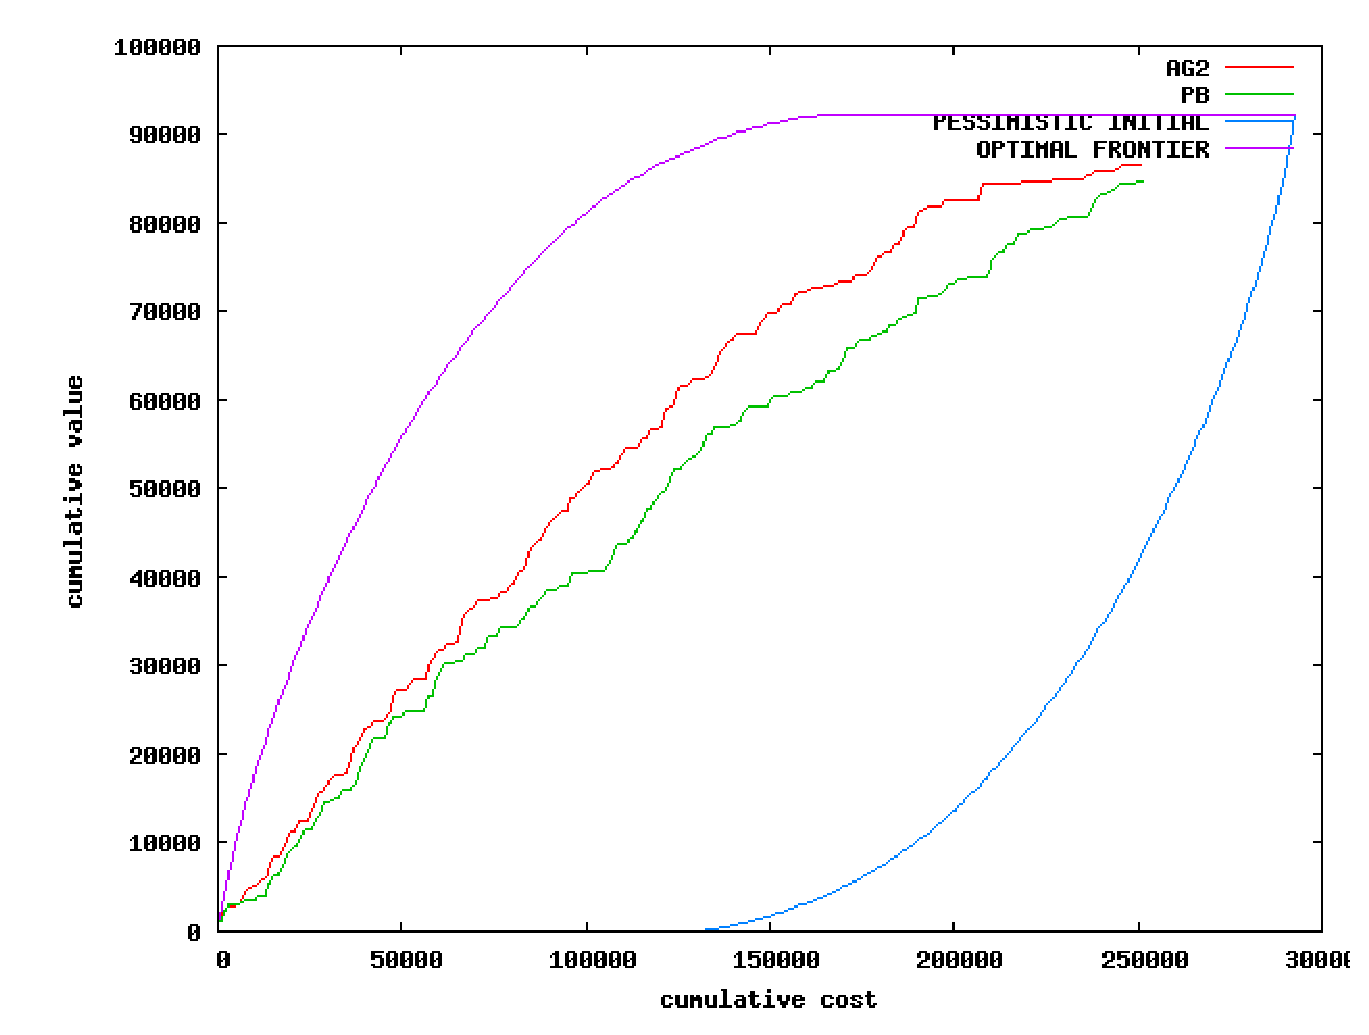
\includegraphics[width=5.35cm]{fakechart.eps}
      \end{minipage}
      \begin{minipage}{7.65cm}
        \begin{equation}\label{eq:score}
          \mathtt{score} = \frac{\int AC - \int PF}{\int OF - \int PF}
        \end{equation}
        By using the area between the OF and PF curve, the project configuration bears no impact on the final score. Thus leaving just the impact of the model inputs and prioritization policy.
      \end{minipage}
    }
\end{kasten}

\begin{kasten}
    \section*{ \hspace{0.1cm} {\color{red} \underline{MODEL INPUTS}}}
    \large{
    POM2 accepted eight input variables.  \textit{Criticality}: affects 
requirements development cost.  \textit{Criticality Modifier}: affects 
the severity of criticality. \textit{Culture}: affects requirements 
reordering and perceived value.  \textit{Initial-known}: sets the
size of the initial requirements set.  \textit{Inter-dependency}: 
frequency of inter-team dependency for requirements.  \textit{Size}: 
size of project (number of requirements).  \textit{Team size}: size of teams 
working on project.  \textit{Dynamism}: how frequently requirements' values 
change.

    }
\end{kasten}

\begin{kasten}
    \section*{ \hspace{0.1cm} {\color{red} \underline{RESULTS}}}
    \tiny
    
\begin{tabular}{@{ } l @{ } r | @{ } r | @{ } r | @{ } r | @{ } r | @{ } r | @{ } r | @{ } r | @{ } r | @{ } r | @{ } r |}
% \multicolumn{2}{c|}{~}&\multicolumn{10}{c}{Note: ranges run $bin_{i} <= value < bin_{i+1}$}\\
%\multicolumn{2}{c|}{~} \\
%\multicolumn{2}{c|}{~} \\
\cline{3-12}
  	&& bin 1 & bin 2 & bin 3 & bin 4 & bin 5 & bin 6 & bin 7 & bin 8 & bin 9 & bin 10 \\
          \cline{2-12}
%          & & & & & & & & & & & \\
	  & criticality
	  & .82
	  & .86
	  & .91
	  & .95
	  & 1.0
	  & 1.04
	  & 1.08
	  & 1.13
	  & 1.17
	  & 1.22\\
	  & criticality modifier
  	  & 2.0
	  & 2.8
	  & 3.6
	  & 4.4
	  & 5.2
	  & 6.0
	  & 6.8
	  & 7.6
	  & 8.4
	  & 9.2\\
	  &culture
	  & 0
	  & 10
	  & 20
	  & 30
	  & 40
	  & 50
	  & 60
	  & 70
	  & 80
	  & 90 \\
	  &initial known
	  & .40
	  & .43
	  & .46
	  & .49
	  & .52
	  & .55
	  & .58
	  & .61
	  & .64
	  & .67\\
	  &inter-dependency
	  & 0
	  & 10
	  & 20
	  & 30
	  & 40
	  & 50
	  & 60
	  & 70
	  & 80
	  & 90\\
	  &size (total personnel)
	  & 3.0
	  & 32.7
	  & 62.4
	  & 92.1
	  & 121.8
	  & 151.5
	  & 181.2
	  & 210.9
	  & 240.6
	  & 270.3\\
policy / dynamism&team size (people per team)
	  & 1.0
	  & 5.1
	  & 9.2
	  & 13.3
	  & 17.4
	  & 21.5
	  & 25.6
	  & 29.7
	  & 33.8
	  & 37.9\\
          

%policy / dynamism \\
\hline
plan-based / very low&criticality&
 &
 &
 &
 &
 &
 &
 &
 &
 &
 \\
$\sigma=\lambda=0$&criticality modifier&
 &
 &
 &
 &
 &
 &
 &
 &
 &
 \\
&culture&
 &
 &
 &
 &
 &
 &
 &
 &
 &
 \\
&initial known     &
 &
 &
 &
 &
 &
 &
 &
 &
\sq{2}{98} &
\sq{4}{96} \\
&inter-dependency     &
 &
 &
 &
 &
 &
 &
\sq{1}{99} &
\sq{1}{99} &
\sq{1}{99} &
 \\
&size     &
\sq{89}{11} &
\sq{2}{98} &
 &
 &
 &
 &
 &
 &
 &
 \\
&team size     &
 &
 &
 &
 &
 &
 &
 &
 &
 &
\sq{1}{99} \\
          \hline
 plan-based / medium&criticality     &
 &
 &
 &
 &
 &
 &
 &
\sq{5}{95} &
\sq{21}{79} &
\sq{52}{48} \\
$\sigma = 0.15, \lambda = 0.0.15$&criticality modifier&
 &
 &
 &
 &
 &
 &
 &
 &
 &
 \\
&culture&
 &
 &
 &
 &
 &
 &
 &
 &
 &
 \\
&initial known&
 &
 &
 &
 &
 &
 &
 &
 &
 &
 \\
&inter-dependency     &
 &
 &
 &
 &
 &
\sq{1}{99} &
\sq{2}{98} &
\sq{6}{94} &
\sq{6}{94} &
\sq{8}{92} \\
&size&
 &
 &
 &
 &
 &
 &
 &
 &
 &
 \\
&team size     &
 &
 &
 &
 &
 &
 &
 &
 &
 &
\sq{1}{99} \\
          \hline
plan-based / very-high &criticality     &
 &
 &
 &
 &
 &
 &
\sq{1}{99} &
\sq{6}{94} &
\sq{22}{78} &
\sq{58}{42} \\
$\sigma=2, \lambda=0.2$&criticality modifier&
 &
 &
 &
 &
 &
 &
 &
 &
 &
 \\
&culture&
 &
 &
 &
 &
 &
 &
 &
 &
 &
 \\
&initial known&
 &
 &
 &
 &
 &
 &
 &
 &
 &
 \\
&inter-dependency     &
 &
 &
 &
 &
 &
\sq{2}{98} &
\sq{3}{97} &
\sq{6}{94} &
\sq{10}{90} &
\sq{11}{89} \\
&size&
 &
 &
 &
 &
 &
 &
 &
 &
 &
 \\
&team size     &
 &
 &
 &
 &
 &
 &
 &
 &
 &
\sq{1}{99} \\
          \hline
agile 2 / very low&criticality&
 &
 &
 &
 &
 &
 &
 &
 &
 &
 \\
$\sigma=\lambda=0$&criticality modifier&
 &
 &
 &
 &
 &
 &
 &
 &
 &
 \\
&culture&
 &
 &
 &
 &
 &
 &
 &
 &
 &
 \\
&initial known     &
 &
 &
 &
 &
 &
 &
\sq{1}{99} &
\sq{4}{96} &
\sq{12}{88} &
\sq{27}{73} \\
&interdependency     &
 &
 &
 &
 &
 &
\sq{1}{99} &
\sq{4}{96} &
\sq{6}{94} &
\sq{5}{95} &
\sq{3}{97} \\
&size     &
\sq{72}{28} &
\sq{1}{99} &
 &
 &
 &
 &
 &
 &
 &
 \\
&team size     &
 &
 &
 &
 &
 &
 &
 &
 &
\sq{1}{99} &
\sq{4}{96} \\
\hline
agile 2 / medium&criticality     &
\sq{1}{99} &
 &
 &
 &
 &
 &
\sq{1}{99} &
\sq{1}{99} &
\sq{1}{99} &
\sq{1}{99} \\
$\sigma=0.15, \lambda=0.015$&criticality modifier     &
 &
 &
 &
 &
 &
 &
\sq{1}{99} &
\sq{1}{99} &
\sq{1}{99} &
\sq{1}{99} \\
&culture     &
 &
 &
 &
 &
 &
\sq{3}{97} &
\sq{10}{90} &
\sq{19}{81} &
\sq{22}{78} &
\sq{29}{71} \\
&initial known     &
 &
 &
 &
 &
\sq{1}{99} &
 &
\sq{2}{98} &
\sq{2}{98} &
\sq{2}{98} &
\sq{2}{98} \\
&interdependency     &
 &
 &
 &
\sq{1}{99} &
\sq{1}{99} &
\sq{1}{99} &
\sq{1}{99} &
 &
\sq{1}{99} &
 \\
&size     &
\sq{97}{3} &
 &
 &
 &
 &
 &
 &
 &
 &
 \\
&team size     &
 &
\sq{17}{83} &
\sq{20}{80} &
\sq{11}{89} &
\sq{6}{94} &
\sq{1}{99} &
 &
 &
 &
 \\
          \hline
agile 2 / very high&criticality     &
\sq{1}{99} &
 &
 &
 &
\sq{1}{99} &
 &
\sq{1}{99} &
\sq{1}{99} &
\sq{1}{99} &
\sq{1}{99} \\
$\sigma=2, \lambda=0.2$&criticality modifier     &
\sq{1}{99} &
\sq{1}{99} &
\sq{1}{99} &
\sq{1}{99} &
\sq{1}{99} &
\sq{1}{99} &
\sq{1}{99} &
 &
\sq{1}{99} &
\sq{1}{99} \\
&culture     &
 &
 &
 &
 &
\sq{1}{99} &
\sq{4}{96} &
\sq{13}{87} &
\sq{17}{83} &
\sq{20}{80} &
\sq{22}{78} \\
&initial known     &
 &
 &
 &
 &
 &
\sq{1}{99} &
\sq{1}{99} &
\sq{1}{99} &
\sq{1}{99} &
\sq{1}{99} \\
&interdependency     &
 &
\sq{1}{99} &
\sq{1}{99} &
\sq{1}{99} &
\sq{1}{99} &
\sq{1}{99} &
\sq{1}{99} &
\sq{1}{99} &
 &
\sq{1}{99} \\
&size     &
\sq{100}{0} &
 &
 &
 &
 &
 &
 &
 &
 &
 \\
&team size     &
 &
\sq{15}{85} &
\sq{18}{82} &
\sq{11}{89} &
\sq{5}{95} &
\sq{2}{98} &
\sq{1}{99} &
 &
 &
\\
\end{tabular}


    \vspace{-.5em}
\end{kasten}

    \end{spalte}
%%%%%%%%%%%%%%%%%%%%%%%%%%%%%%%%%%%%%%%%%%%%%%%%%%%%
%%%               fourth column                  %%%
%%%%%%%%%%%%%%%%%%%%%%%%%%%%%%%%%%%%%%%%%%%%%%%%%%%%
    \begin{spalte}
		\begin{kasten}
    \section*{ \hspace{0.1cm} {\color{red} \underline{HOW WE SEARCH THE MODEL}}}
    \vspace{-0.5em}
    \begin{minipage}{5cm}
      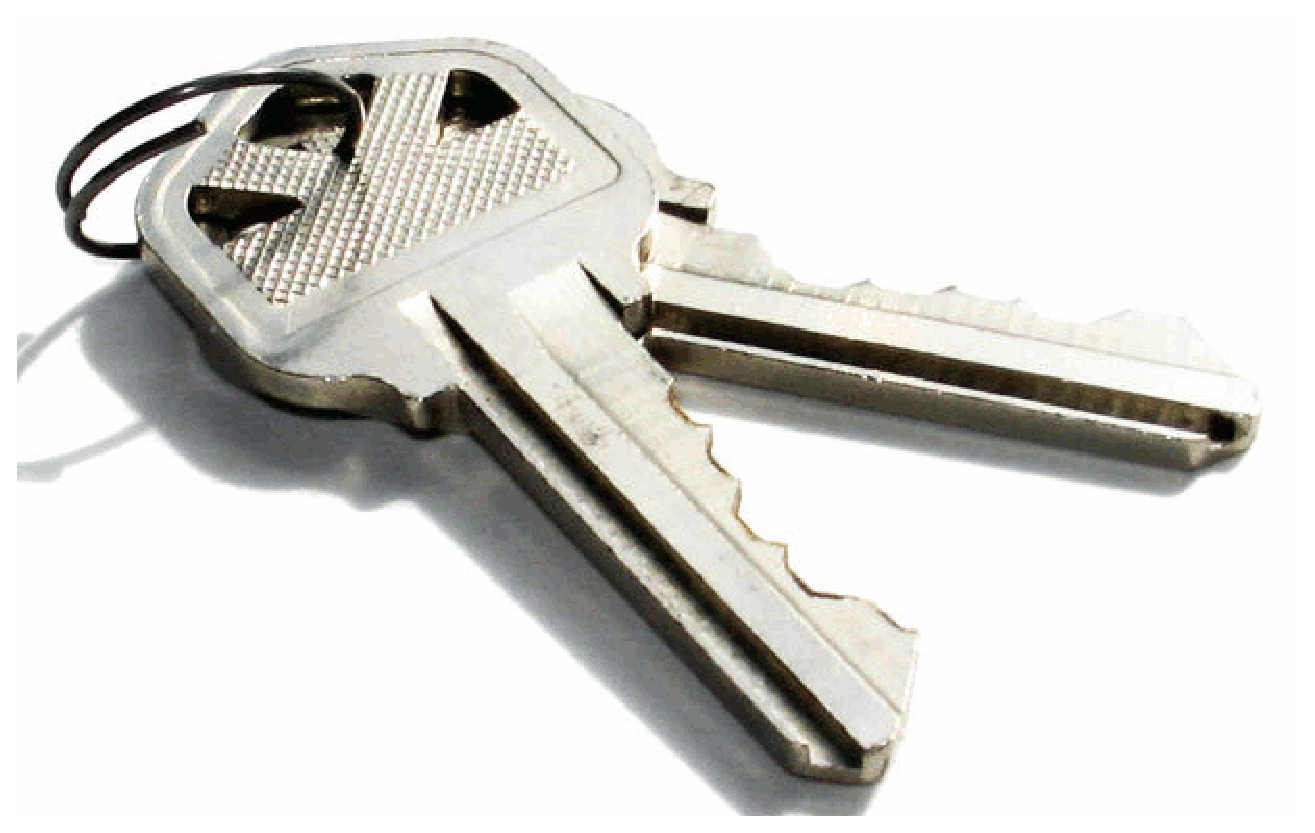
\includegraphics[width=5cm]{keys.eps}
    \end{minipage}
    \begin{minipage}{8cm}
      \large{
        POM2 presents a 10 dimensional hypothesis space. To find the critical factors, POM2 uses the KEYS range subset selector. KEYS uses Bayesian contrast set learning to find the single range that most selects for the preferred outcomes. Subsequent iterations of KEYS constrains the simulator to 

      }
    \end{minipage}
    \large{
always include that range. The smallest subset of selected ranges that most improve the final output is the {\em model treatment}.
    }
    \vspace{-0.5em}
\end{kasten}

\begin{kasten}
    \section*{ \hspace{0.1cm} {\color{red} \underline{WHAT WE FOUND}}}
    \vspace{-0.5em}
    \large{
      \begin{minipage}{4.5cm}
          \begin{center}
            {\small{
            Low dynamism: $\sigma=0, \lambda=0$
            
            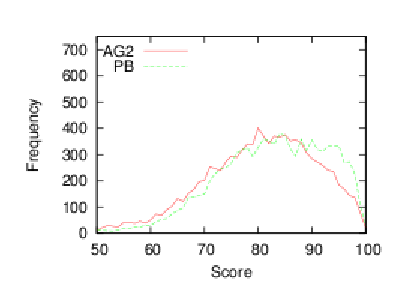
\includegraphics[width=4.5cm]{fr-v-sc-msvl.eps}
            
            Medium dynamism: $\sigma=0.15, \lambda=0.015$
            
            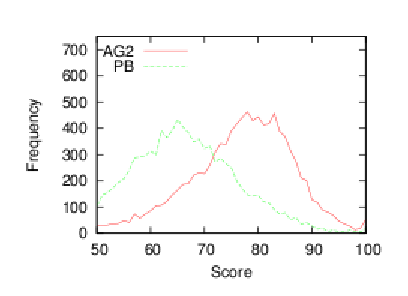
\includegraphics[width=4.5cm]{fr-v-sc-msmi.eps}
            
            High dynamism: $\sigma=2, \lambda=0.2$
            
            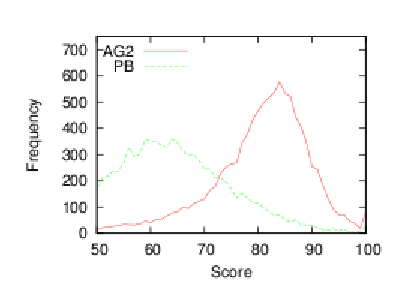
\includegraphics[width=4.5cm]{fr-v-sc-msvh.eps}
            }}
          \end{center}
      \end{minipage}
      \begin{minipage}{8.5cm}
        We ran KEYS 1000 times for each combination of {very low, medium, very high} dynamism and {plan-based, agile 2} prioritization policy. The findings are summarized in \S{RESULTS}. Several majority case effects deserve note:
        \vspace{-0.8em}
        \begin{verysmallitem}
        \item Criticality Modifier: Never chosen in more than $1\%$ of the cases.
        \item Initial Known$/$Inter-Dependency: Never chosen in $>50\%$ of the runs.
        \item Team Size: Never $<5$ team members.
        \item For Agile 2:
          \vspace{-0.7em}
          \begin{verysmallitem}
          \item Size: The smallest size was chosen in $72\%-100\%$ of the runs.
          \item Culture: The upper bins were chosen in $72\%-80\%$ of the runs where dynamism was a factor.
          \item Team Size: Should be 5 - 17 for medium and very high dynamism.
          \end{verysmallitem}
        \end{verysmallitem}

\vspace{-0.8em}
The 1000 runs of KEYS shows that many
results are very similar (e.g. all the Agile 2
          results offer nearly the same pattern). 
KEYS shows that there are two major divisions of 
its 10-dimensional space: very high criticality 
and very small team size. We ran 10,000 
simulations in the union of these two divisions
      \end{minipage}
    }

 (shown above). The median score of Agile 
2 is shows stability under changing dynamism, while 
the median score of Plan-Based falls  as dynamism increases. We see that the median score of Agile 2 is equal to or greater than the median score of Plan-Based development.

    \vspace{3mm}
    We conclude that in the general case, Agile 2 out performs Plan-Based development. Only rarely does Plan-Based out perform Agile 2.
    \vspace{-0.1em}
\end{kasten}

\begin{kasten}
  \section*{ \hspace{0.1cm} {\color{red} \underline{RECOMMENDATIONS}}}
    \vspace{-0.5em}
  \large
  \begin{smallenum}
    \item The default development practice should be an Agile 2 method.
    \item Debates about software process can be greatly shortened, and
      improved, by combining process simulation and  AI search.
  \end{smallenum}
    \vspace{-0.5em}
\end{kasten}

\begin{kasten}
    \section*{ \hspace{0.1cm} {\color{red} \underline{FOR MORE INFORMATION}}}
    \vspace{-0.5em}
    \normalsize{
      Bryan Lemon (\url{bryan@bryanlemon.com})\\
      Tim Menzies Ph.D. (\url{tim@menzies.us})\\
      %Justin Price (\url{justin.n.price@gmail.com})\\
      Joseph D'Alessandro (\url{jdalessa57@gmail.com})
    }
    \vspace{-0.5em}
\end{kasten}

\begin{kasten}
    \section*{ \hspace{0.1cm} {\color{red} \underline{SUPPORT}}}
    \vspace{-0.5em}
    \large{
      \begin{minipage}{2cm}
        
\includegraphics[width=2cm]{nsf_logo.eps}
      \end{minipage}
      \begin{minipage}{11cm}
This research was carried out at West Virginia
University under a grant from the National Science Foundation (NSF CISE 71608561).
      \end{minipage}
    }
\end{kasten}

    \end{spalte}
    }
    \end{lrbox}
\resizebox*{0.98\textwidth}{!}{%
  \usebox{\spalten}}\hfill\mbox{}\vfill
\end{document}


